\documentclass[12pt, aspectratio=43]{beamer}
\usepackage[backend=bibtex, style=authoryear]{biblatex} % bibliography
\usepackage{multirow}
\usepackage{adjustbox}

% BEAMER TEMPLATE AND THEME
\setbeamertemplate{footline}[frame number]
\usetheme{Estonia}
\mode<presentation>
\AtBeginSection[]{
  \begin{frame}
  \vfill
  \centering
  \begin{beamercolorbox}[sep=8pt,center,shadow=true,rounded=true]{title}
    \usebeamerfont{title}\insertsectionhead\par%
  \end{beamercolorbox}
  \vfill
  \end{frame}
}

\addbibresource{../biblio.bib}

% TITLE PAGE
\title{Kubernetes cluster simulator based on Batsim}
\title{Development and evaluation of a Kubernetes cluster simulator based on
Batsim}

\author{\textbf{Presented by:} Théo Larue\\\textbf{Supervised by:} Olivier
Richard \& Michael Mercier}

\date{August 31, 2020}

\institute[Théo LARUE]{Université Grenoble Alpes}

\titlegraphic{
	\includegraphics[height=5ex]{../imgs/uga-logo.png}\hspace{2ex}
	\includegraphics[height=6ex]{../imgs/ENSIMAG.png}\hspace{2ex}
	\includegraphics[height=5ex]{../imgs/Logo-LIG.jpg}\hspace{2ex}
	\includegraphics[height=5ex]{../imgs/ryax-logo.png}
}

\begin{document}

\frame{\titlepage}

\begin{frame}\frametitle{Table of contents}\tableofcontents
\end{frame}

\section{Introduction}

\begin{frame}{Computer infrastructure}
	TODO: definition of a computer infrastructure

	\includegraphics[scale=0.3]{../imgs/comp-infra-michael.png}
	\small{Placeholder (from michael thesis). TODO: my own illustration}
\end{frame}

\begin{frame}{Resource and Jobs Management System}
	TODO: the RJMS is at the core of the hpc cluster.

	def or diagram illustrating a RJMS (without much details). Show that the
	scheduler is part of the RJMS.

	Examples: OAR, Apache Mesos, hadoop YARN, SLURM
\end{frame}

\begin{frame}{Kubernetes}
	Explain containers real quick.

	Container orchestration software, description based.
\end{frame}

\begin{frame}{Studying computer infrastructures}
	\begin{columns}
		\column{0.5\textwidth}
		\begin{exampleblock}{Objects of studies}
			\begin{itemize}
				\item Workloads
				\item Applications
				\item System size
				\item Network topology
				\item Scheduling policies
			\end{itemize}
		\end{exampleblock}

		\column{0.5\textwidth}
		\begin{block}{How ?}
			\begin{itemize}
				\item Analytical study
				\item Real experiments
				\item Emulation
				\item Simulation
			\end{itemize}
		\end{block}
	\end{columns}
	%How to study these infra? Too many elements and interactions to
	%consider, so no theoretical study. 

	%Real experiments are too costly (both in time and resources) and not
	%reproducible.

	%Note: revoir ref sur les interactions inattendues entre scheduler et
	%queues
\end{frame}

\begin{frame}{Batsim}
	Aimed at studying RJMS.

	Strong decoupling decision process / simulator.
\end{frame}

\begin{frame}{The scheduling problem}
	\centering
	\includegraphics[width=0.8\textwidth]{../imgs/gantt_small.png}
	\textbf{Scheduling} is the act of allocating tasks to resources.
\end{frame}

\begin{frame}{Contribution}
	TODO: Our contribution is Batkube, an interface between Batsim and
	Kubernetes schedulers
\end{frame}

\section{Literature review}
\begin{frame}{Domain specific simulators}
	refs on domain specific simulators 
\end{frame}

\begin{frame}{Software specific simulators}
	YARNSim, SLURM simulator
\end{frame}

\begin{frame}{Publication specific simulators}
	``Publish and perish'' - Milian Poquet
\end{frame}

\begin{frame}{SimGrid}
	SimGrid: Versatile, scalable, accurate.

	Cpu = a computation speed.\\
	Storage = a seek time and a data transfert rate.\\
	Network = a flow model, modeling bandwith sharing behaviors.

	Simple models but thoroughly validated.
\end{frame}


\begin{frame}{Related work}
	GridSim

	Alea: modular, extensible.

	Accasim: supports additional information (temperature, power
	consuption). Very efficient in terms of simulation time and memory
	usage.
\end{frame}

\begin{frame}{Kubernetes cluster simulation}
	k8s-cluster-simulator: open source, student project, delay jobs.
	Schedulers provided via a Go interface.

	joySim: closed-source, fully fledged kubernetes cluster simulator,
	service oriented (mock nodes).
\end{frame}

\section{Integrating Kubernetes schedulers to Batsim}

\begin{frame}{Technical challenges}
	\begin{alertblock}{Challenges to tackle}
		\begin{enumerate}
				\uncover<1->{\item Integration with Kubernetes.}
				\uncover<2->{\item Intercepting scheduler time.}
				\uncover<3->{\item Time synchronization between Batsim and the scheduler.}
		\end{enumerate}
	\end{alertblock}
\end{frame}

\begin{frame}{Batsim concepts}
	\begin{columns}
		\column{0.5\textwidth}
		\centering
		\includegraphics[width=\textwidth]{../imgs/batsim-sequence-diag.png}
		\tiny{source \url{https://batsim.readthedocs.io}}

		\column{0.5\textwidth}
		Batsim events and protocol.

		User defined workloads.

		(insert json examples?)
\end{columns}
\end{frame}

\begin{frame}{Kubernetes concepts}
	\centering
	\only<1>{\includegraphics[width=\textwidth]{../imgs/components-of-kubernetes.png}}
	\only<2>{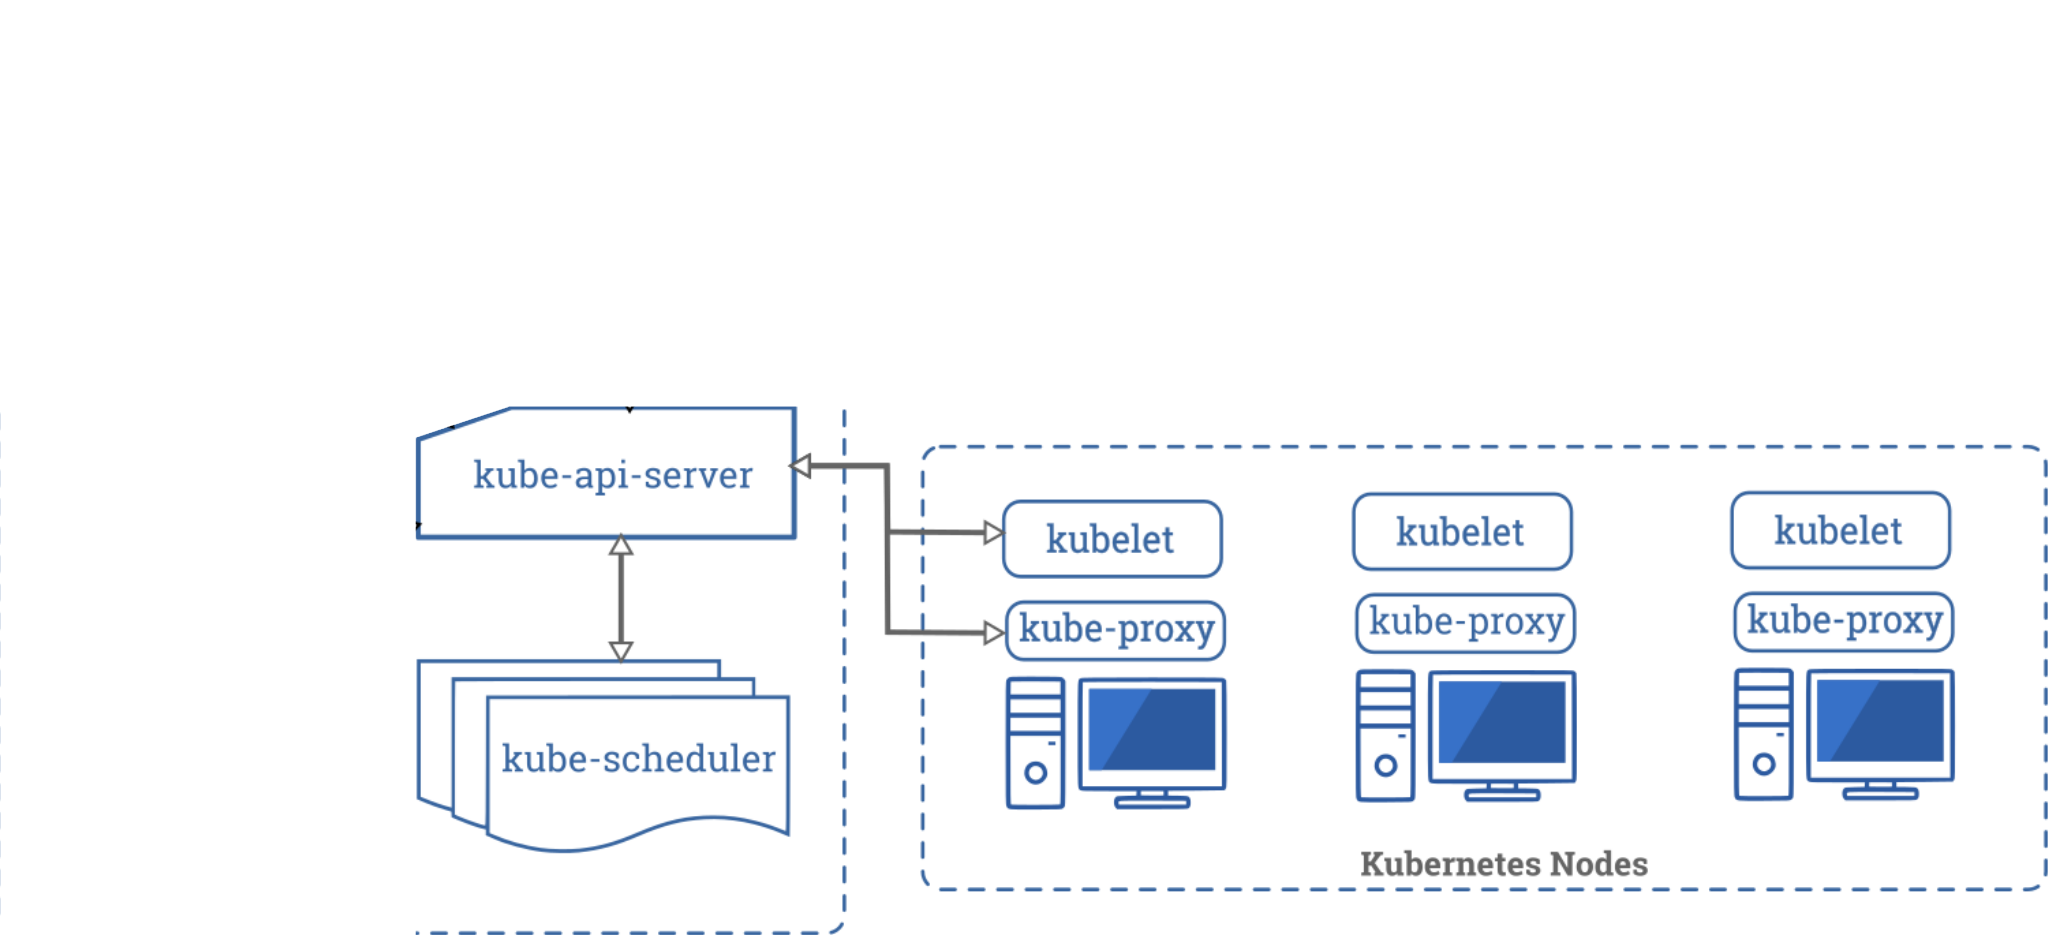
\includegraphics[width=\textwidth]{../imgs/components-of-kubernetes-2.png}}
	\tiny{source: \url{https://kubernetes.io/docs/concepts/overview/components/}}\\
	\small{Kubernetes components.}
\end{frame}

\begin{frame}{Different paradigms}
	Batsim: event based, simulation time.

	Kubernetes scheduler: asynchronous calls to the API, machine time.

	The goal is to make the scheduler event based and relying on simulation
	time for Batsim, and make Batsim a kube-api-server to the scheduler.
\end{frame}

\begin{frame}{Batkube integration with Kubernetes}
	\centering
	\includegraphics[width=0.8\textwidth]{../imgs/custom-api.pdf}\\
	\small{Reimplementation of a custom API.}
\end{frame}

\begin{frame}{Architeture of Batkube}
	\centering
	\includegraphics[width=\textwidth]{../imgs/batkube-architecture-3-synchro.pdf}
	\small{Global architecture of Batkube.}
\end{frame}

%\begin{frame}{Similar resources}
%	\begin{columns}
%		\column{0.5\textwidth}
%		\centering
%		\includegraphics[width=\textwidth]{../imgs/node-overview.png}
%		\tiny{source: \url{https://kubernetes.io/docs/tutorials/kubernetes-basics/explore/explore-intro/}}
%
%		\column{0.5\textwidth}
%		\begin{block}{Translation between Kubernetes and Batsim}
%			\begin{itemize}
%				\item A Pod = a job.
%				\item A Node = a compute resource.
%			\end{itemize}
%		\end{block}
%	\end{columns}
%\end{frame}

\begin{frame}{Time interception}
	\centering
	\includegraphics[width=0.6\textwidth]{../imgs/synchro-go-sources.pdf}\\
	\small{Schedulers are patched to redirect their time.}
\end{frame}

%\begin{frame}{batsky-go}
%	\begin{columns}
%		\column{0.5\textwidth}
%		\centering
%		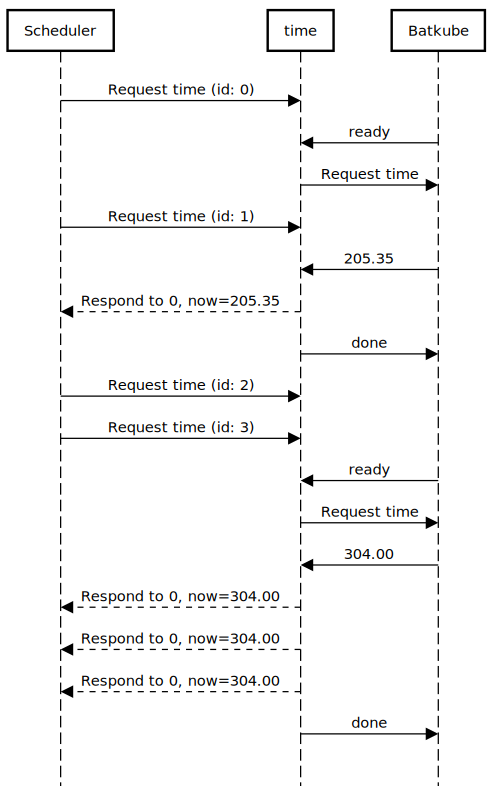
\includegraphics[scale=0.38]{../imgs/requester-broker.pdf}
%		
%		\column{0.5\textwidth}
%		Exchanges between the scheduler, batsky-go (``time'') and Batsim
%	\end{columns}
%\end{frame}

\begin{frame}[allowframebreaks]{Time synchronization}
	TODO: explain CML
	\framebreak

	\centering
	\includegraphics[width=0.87\textwidth]{../imgs/lignes_de_temps_simple.pdf}\\
	\small{Time synchronization between Batsim and the scheduler}
\end{frame}

\begin{frame}[allowframebreaks]{Parameters of the synchronization}
		\centering
		\includegraphics[width=0.87\textwidth]{../imgs/timeout.pdf}\\
		Timeout value

		\includegraphics[width=0.8\textwidth]{../imgs/max-timestep.pdf}\\
		Simulation time step $\in$ [\texttt{base-simulation-timestep}, \texttt{max-simulation-timestep}]
\end{frame}

\begin{frame}{Time synchronization breakdown}
	\centering
	\includegraphics[width=0.87\textwidth]{../imgs/lignes_de_temps.pdf}\\
	\small{Time synchronization between Batsim and the scheduler}
\end{frame}

\section{Study of the simulator}

\begin{frame}{Experimental design}
	TODO: Scheduler used, platforms and workloads tested, what experiments (parameters, metrics studied, repetitions)
	%\centering
	%\begin{tabular}{|c|c|c|c|c|c|}
	%	\hline\\
	%	name & number of jobs & jobs type & sub time & resource requests & platform
	%	\hline\\
	%	burst & 200 & delay (170s) & at time zero & 1 cpu & 16x1\\
	%	spaced & 200 & delay (170s) & every ten seconds & 1 cpu & 16x1\\
	%\end{tabular}
\end{frame}

\begin{frame}[allowframebreaks]{Timeout}
	\centering
	\includegraphics[width=\textwidth]{../imgs/timeout_burst_spaced.png}
	\includegraphics[width=\textwidth]{../imgs/timeout_realistic.png}
\end{frame}

\begin{frame}[allowframebreaks]{Maximum simulation timestep}
	\centering
	\includegraphics[width=\textwidth]{../imgs/max-timestep_burst_sp.png}
	\includegraphics[width=\textwidth]{../imgs/max-timestep_realistic.png}
\end{frame}

\begin{frame}{Experimentation on a real cluster}
	\centering
	\includegraphics[width=0.8\textwidth]{../imgs/expe-protocole-v2.pdf}
\end{frame}

\begin{frame}{Deviation with reality}
	\centering
	\begin{adjustbox}{max width=\textwidth}
		\begin{tabular}{|c|c|c|c|c|c|c|c|c|}
			\hline

			\multirow{3}{*}{workload} & \multicolumn{4}{c|}{\textbf{makespan}} & \multicolumn{4}{c|}{\textbf{mean waiting time}}\\

			\cline{2-9}

			& \multicolumn{2}{c|}{emulated} &
			\multicolumn{2}{c|}{simulated} & \multicolumn{2}{c|}{emulated}
			& \multicolumn{2}{c|}{simulated} \\

			\cline{2-9}

			& $\mu$ & $\sigma$ & $\mu$ & $\sigma$ & $\mu$ & $\sigma$ & $\mu$ & $\sigma$ \\

			\hline

			burst & 2467 & 28.3 & 2215 (-252) & 0.508 & 1077 & 10.6 & 970 (-107) & 12.6 \\
			spaced & 2468 & 5.14 & 2257 (-211) & 16.9 & 146 & 1.67 & 48.1 (-97.9) & 9.44 \\
			realistic & 32556 & - & 32555 (-1) & 1.30 & 2884 & - & 2020 (-864) & 950 \\
			\hline
		\end{tabular}
	\end{adjustbox}
\end{frame}

\begin{frame}{Conclusion}
	Deviation with reality: can be fixed with some work on the api. Need
	experiments to measur and quantify this deviation.

	max timestep: studying max timestep alone is not enough, need to study
	it with backoff multiplier.

	base time step: need an experiment on it. Too much importance was
	credited to max timestep, the base timestep might have importance.
\end{frame}

\section{Discussion and future work}
\begin{frame}{Capabilities and limitations of Batkube}
	WIP
	\begin{columns}
		\column{0.5\textwidth}
		\begin{block}{Capabilities}
			\begin{itemize}
				\item Delay jobs
				\item Cpu and memory requests
				\item Can patch any kubernetes scheduler written in Go
				\item The api only supports the default scheduler
			\end{itemize}
		\end{block}

		\column{0.5\textwidth}
		\begin{alertblock}{Limitations}
			\begin{itemize}
				\item Memory hungry (in fact, the scheduler is memory hungry)
				\item Some problems with the scheduler
				\item Not scalable
			\end{itemize}
		\end{alertblock}
	\end{columns}
\end{frame}

\begin{frame}{Perspectives for future work}
	- parallel jobs\\
	- storage\\
	- more complete api: support for more schedulers but also tools (monitoring tools)
\end{frame}

\begin{frame}[allowframebreaks]
        \frametitle{References}
	\printbibliography
\end{frame}

\end{document}
